\documentclass{standalone}

\usepackage{tikz}
\usetikzlibrary{automata,positioning}
\begin{document}
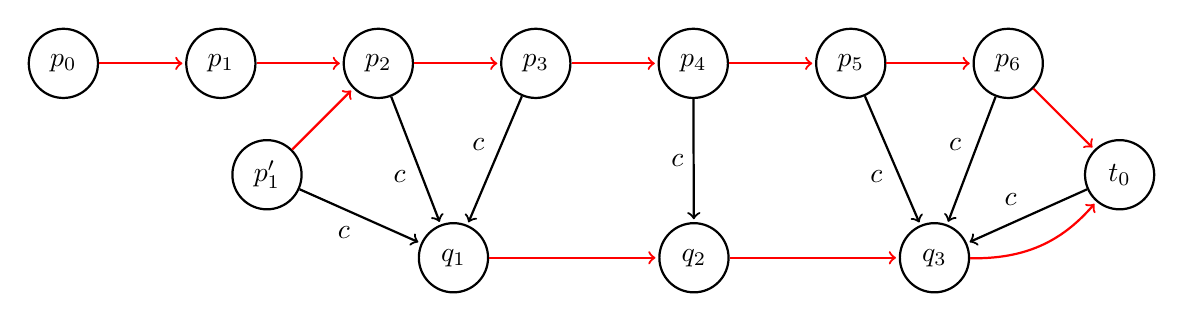
\begin{tikzpicture}[shorten >=1pt,node distance=2cm,on grid,auto,scale=2,thick] 
    \node[state] (p_0) {$p_0$};
    \node[state] (p_1) [right=of p_0] {$p_1$};
    \node[state] (p_2) [right=of p_1] {$p_2$};
    \node[state] (p_3) [right=of p_2] {$p_3$};
    \node[state] (p_4) [right=of p_3] {$p_4$};
    \node[state] (p_5) [right=of p_4] {$p_5$};
    \node[state] (p_6) [right=of p_5] {$p_6$};
    \node[state] (p_1p) [below left=of p_2] {$p_1'$};
    \node[state] (t_0) [below right=of p_6] {$t_0$};
    \node[state] (q_3) [left=of t_0, xshift=-1em, yshift=-3em] {$q_3$};
    \node[state] (q_2) [left=of q_3, xshift=-3em] {$q_2$};
    \node[state] (q_1) [left=of q_2, xshift=-3em] {$q_1$}; 
    \path[->,red] 
        (p_0) edge (p_1) 
        (p_1) edge (p_2) 
        (p_2) edge (p_3) 
        (p_3) edge (p_4)
        (p_4) edge (p_5)
        (p_5) edge (p_6)
        (p_6) edge (t_0)
        (q_1) edge (q_2)
        (q_2) edge (q_3)
        (q_3) edge [bend right=25] (t_0)
        (p_1p) edge (p_2);
    \path[->]
        (p_2) edge [swap] node {$c$} (q_1)
        (p_3) edge [swap] node {$c$} (q_1)
        (p_4) edge [swap] node {$c$} (q_2)
        (p_5) edge [swap] node {$c$} (q_3)
        (p_6) edge [swap] node {$c$} (q_3)
        (t_0) edge [swap] node {$c$} (q_3)
        (p_1p) edge [swap] node {$c$} (q_1);
\end{tikzpicture}
\end{document}  